\textcolor[rgb]{1.00,0.00,0.00}{Although mbCRT algorithm enables control with regression trees-based models, it suffers from two significant limitations:
\begin{enumerate}[leftmargin=1cm]
	\item It is based on uni-variate output regression tree models and is unable to make multi-variate predictions. 
	\item It is a `one-step lookahead' algorithm and can account for an unexpected disturbance only one time-step before it occurs, thus making it sub-par as compared to receding horizon control algorithms.
\end{enumerate}
The finite receding horizon control approach involves optimizing a cost function subject to the dynamics of the system and the constraints, over a finite horizon of time. After an optimal sequence of control inputs is computed, only the first input is applied to the system, then at the next step the optimization is solved again considering the new measurements, as shown in Fig. \ref{F:MPC-illust}.} 
\begin{figure}
	\centering
	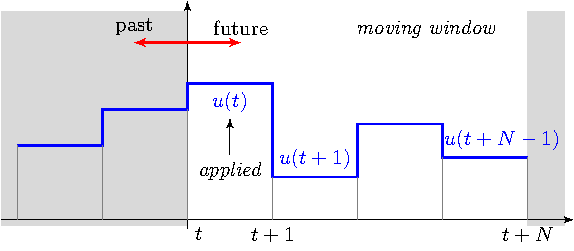
\includegraphics[scale=0.85]{Figures/receding_horizon.pdf}
	\caption{Finite-horizon moving window of MPC: at time $t$, the MPC optimization problem is solved for a finite length window of $N$ steps and the first control input $u(t)$ is applied; the window then recedes one step forward and the process is repeated at time $t+1$.}
	\captionsetup{justification=centering}
	\label{F:MPC-illust}
\end{figure} 
\textcolor[rgb]{1.00,0.00,0.00}{Our main goal is to construct data-driven predictive models for cyber-physical systems that relates the value of the response variable with the values of the predictor variables or features over an horizon with an arbitrary length $N$, and that can be used to setup a receding horizon control problem. In this way we substantially improve the simple mbCRT modeling framework.}

\textcolor[rgb]{1.00,0.00,0.00}{Regression trees-based methods are \emph{predominantly} uni-variate output, i.e. defined only for single output variable. We introduce a different splitting criteria for trees which enables us to predict multiple outputs. If we consider these new outputs as the future states of the single output system, the multi-output tree enables us to implement receding horizon control as the prediction can be made for multiple steps. For example, in a building automation case study, one can consider a training dataset with information about the building states like zone temperatures, control set-points and weather conditions, while the output could represented by the power consumption of the building. With a single output model, one could estimate the power consumption of the building only at time-step $t$. The approach we propose allows to predict the power consumption of the same building at multiple time-steps, i.e. considering a tree with $N+1$ outputs, one could estimate power consumption of the building at $t, t+1,\ldots,t+N$. This is termed as lookahead capability of a multi-variate output tree. A related case study will be considered in Sec. \ref{sec:case}. In this section, we first explain how the regression trees learning algorithm CART is built, and then modify it into a multi-variate output algorithm to create models that are suitable for finite horizon prediction. Finally, we setup a receding horizon control problem based on such models.}

\subsection{Predictive modeling with multi-output regression trees}
\label{SS:training_algo}

We use the following notation. We consider a dataset with $n$ observations, where each \textcolor[rgb]{1.00,0.00,0.00}{observation} has $s$ features and model has $N$ outputs as
\textcolor[rgb]{1.00,0.00,0.00}{\begin{align}
& x^i := [\x^i_1, \dots, \x^i_s] \in \mathbb{R}^s \nonumber \\
& y^i := [\y^i_1, \dots, \y^i_N] \in \mathbb{R}^N  \label{E:dataset}\\
& i \in \{1,2,\dots, n\}. \nonumber 
\end{align} }
Splitting of nodes is shown in Fig. \ref{F:RT}. At $i^{\mathrm{th}}$ node, CART splits the data set into 2 subsets. The left branch $R_L$ contains the data corresponding to $\mathrm{x}_j \leq t_j$ and the right branch $R_R$ corresponding to $\mathrm{x}_j > t_j$. The optimal split at each node is then determined by minimizing the sum of mean square error in both the branches:
\begin{gather}
(\x_k,t_k) = \argmin    \sum_{\{i|\x^i \in R_L\}}{(\y^i_1 - \bar{y}_L)^2}  +  \sum_{\{i|\x^i \in R_R\}} {(\y^i_1 - \bar{y}_R)^2}
\label{E:CART_split_rule}
\end{gather}
where $\bar{y}_L$ and $\bar{y}_R$ are the mean outputs of all the data points in $R_L$ and $R_R$, respectively. The tree is grown in this fashion till the number of data points in the terminal nodes (leaves) exceeds the minimum number of observations in a leaf $minLeaf$, which is often a tuning parameter. Typically a tree is grown till $minLeaf$ size is achieved, and then cost-complexity pruning is employed by collapsing the weak splits \cite{HastieTibshiraniFriedmanEtAl2005}.

\begin{figure}
\centering
\subfigure[First split occurs with input $\x^i$ at $t_i$, second split with input $\x^j$ at $t_j$ and so on, resulting in 5 regions in this case $R_1, \dots, R_5$.]{
\label{F:RT}
\centering
\begin{tikzpicture}[->,>=stealth',level/.style={sibling distance = 3.5cm/#1,
  level distance = 1.5cm}] 
\node [branch_c] {}
    child[blue!50!gray!,thick]{ node [branch_l] {}
            child[blue!50!gray!,thick]{ node [branch_l] {$R_1$} edge from parent node[above left] {$\x_j \leq t_j$}}
            child[red!50!gray!,thick]{ node [branch_r] {$R_2$} edge from parent node[above right] {$\x_j > t_j$}} 
            edge from parent node[above left] {$\x_i \leq t_i$}                            
    }
    child[red!50!gray!,thick]{ node [branch_r] {}
            child[blue!50!gray!,thick]{ node [branch_l] {}
            		child[blue!50!gray!,thick]{ node [branch_l] {$R_4$} edge from parent node[above left] {$\x_k \leq t_k$}}
            		child[red!50!gray!,thick]{ node [branch_r] {$R_5$} edge from parent node[above right] {$\x_k > t_k$}} 
            }
            child[red!50!gray!,thick]{ node [branch_r] {$R_3$}}  
            edge from parent node[above right] {$\x_i > t_i$}    
		}
; 
\end{tikzpicture}
}
\subfigure[First split occurs with continuous input $\x_i$ at $t_i$, second split with categorical input $\x_j$ at $t_j^r$ such that $\mathcal{S}_{j,L}=\{ t_j^1,\dots,t_j^r \}$ and $\mathcal{S}_{j,R}=\{ t_j^{r+1},\dots,t_j^q \}$.]{
\label{F:RT2}
\centering
\begin{tikzpicture}[->,>=stealth',level/.style={sibling distance = 3.5cm/#1,
  level distance = 1.5cm}] 
\node [branch_c] {}
    child[blue!50!gray!,thick]{ node [branch_l] {}
            child[blue!50!gray!,dashed,thick]{ node [branch_l] {$R_1$} edge from parent node[above left] {$\x_j \in \mathcal{S}_{j,L}$}}
            child[red!50!gray!,dashed,thick]{ node [branch_r] {$R_2$} edge from parent node[above right] {$\x_j \in \mathcal{S}_{j,R}$}} 
            edge from parent node[above left] {$\x_i \leq t_i$}                            
    }
    child[red!50!gray!,thick]{ node [branch_r] {}
            child[blue!50!gray!,thick]{ node [branch_l] {}
            		child[blue!50!gray!,thick]{ node [branch_l] {$R_4$} edge from parent node[above left] {$\x_k \leq t_k$}}
            		child[red!50!gray!,thick]{ node [branch_r] {$R_5$} edge from parent node[above right] {$\x_k > t_k$}} 
            }
            child[red!50!gray!,thick]{ node [branch_r] {$R_3$}}  
            edge from parent node[above right] {$\x_i > t_i$}    
		}
; 
\end{tikzpicture}
}
\caption{Tree structures for continuous and mix of discrete and continuous variables.}
\captionsetup{justification=centering}
\end{figure}

We extend the same approach to deal with the multi-output data. In order to determine node splits, we are again interested in calculating the splitting variable $\mathrm{x}_k$ and the splitting value $t_k$, but this time we account for errors in all $N$ outputs. Appropriately, we modify \eqref{E:CART_split_rule} as follows:
\begin{gather}
(\mathrm{x}_k,t_k) = \argmin    \sum_{\{i|\x^i \in R_L\}}{||y^i - \bar{y}_L||}_l^2  +  \sum_{\{i|\x^i \in R_R\}} {||y^i - \bar{y}_R||}_l^2
\label{E:DPC_split_rule}
\end{gather}
\textcolor[rgb]{1.00,0.00,0.00}{where $\bar{y}_L,\bar{y}_R \in \mathbb{R}^N$} and represent the mean $\forall y^i \in R_L$ and $\forall y^i \in R_R$, respectively. Norm in this optimization criteria can be chosen to $l^1$ norm if we want to minimize the largest absolute error in the outputs or $l^2$ norm which will minimize the sum of squares across all the outputs. We can also introduce weights matrix \textcolor[rgb]{1.00,0.00,0.00}{$Q \in \mathbb{R}^{N \times N}$} as further tuning parameter and choose a quadratic optimization objective:
\begin{gather}
\label{E:DPC_split_rule2}
(\mathrm{x}_k,t_k) = \argmin    \sum_{\{i|\x^i \in R_L\}}{(y^i - \bar{y}_L)}^TQ{(y^i - \bar{y}_L)}  + \sum_{\{i|\x^i \in R_R\}} {(y^i - \bar{y}_R)}^TQ{(y^i - \bar{y}_R)}.
\end{gather}
Both  \eqref{E:DPC_split_rule} and \eqref{E:DPC_split_rule2} can be solved numerically by discretizing the search space of $t_k$ between $max(\mathrm{x}_k)$ and $min(\mathrm{x}_k)$ calculated across $n$ data points. The finer the resolution, the better the accuracy of splits. The terminating condition for growing the tree remains unchanged in \eqref{E:DPC_split_rule} and \eqref{E:DPC_split_rule2}.

So far, we covered how a tree is built when all the features/variables are continuous. It is often the case that some of the features in the data set are categorical, i.e. they can only take discrete values. 
The problem of partitioning a set of discrete values in two subsets is a combinatorial problem. Consider a categorical input feature $\mathrm{x}_c$ which can take $q$ different values belonging to the set $\mathcal{S}_c=\{t_c^1,\dots,t_c^q \}$. Number of ways to partition $\mathcal{S}_c$ into two non-empty subsets are $2^{q-1}-1$. Note that the different possible partitions scale exponentially with $q$, unlike in the continuous case where it grows linearly with resolution. Hence, when $q$ is large, exact search is not computationally easy to solve. We use a near-optimal approach to narrow down this search over all possible partitions. The approach is simliar to the one described in \cite{Ripley2007} for single-output system. We first find out all $y^i$ corresponding to each element in $\mathcal{S}_c$ and then order the set $\mathcal{S}_c$ according to an increasing mean:
\begin{gather}
\label{E:DPC_cat_split_rule}
\bar{y}_q = \frac{\displaystyle\sum_{\{i|\mathrm{x}_c=t_c^q\}} ||y^i||_l}{N_q},
\end{gather}
where $N_q$ is the number of data points for which $\mathrm{x}_c=t_q$. Once $\mathcal{S}_c=\{t_c^1,\dots,t_c^q \}$ is ordered such that 
$\bar{y}_1< \dots < \bar{y}_q$, we split the variable as if it is a continuous variable using \eqref{E:DPC_split_rule} or \eqref{E:DPC_split_rule2} depending upon the chosen type of formulation. If the cost is minimized for $\mathrm{x}_c \leq t_c^r$, then the left branch contains $\mathrm{x}_c \in \mathcal{S}_{c,L} = \{ t_c^1,\dots,t_c^r \}$ and the right branch contains $\mathrm{x}_c \in \mathcal{S}_{c,R} = \{ t_c^{r+1},\dots,t_c^q \}$. A tree with a mix of continuous and categorical variables is shown in Fig. \ref{F:RT2}. 

In summary, when the dataset contains both types of variables, i.e. continuous and categorical, first the range of all the categorical variables is sorted. 
Then, the optimal cost of splitting is determined for each input feature. 
Finally, the input feature for which this cost is minimum is taken as the splitting variable. Following this approach, we obtain a tree model in the form of
\textcolor[rgb]{1.00,0.00,0.00}{\begin{gather}
[\mathrm{y}_1, \dots, \mathrm{y}_N] = f \left( \mathrm{x}_1, \dots, \mathrm{x}_s \right)
 \label{eq:regtree_multi}
\end{gather}}

\subsection{Predictive control with multi-output regression trees}
\label{SS:control_tree}
\textcolor[rgb]{1.00,0.00,0.00}{In this section we setup a receding horizon control problem using models proposed in \eqref{eq:regtree_multi}. This algorithm is called Data-based Predictive Control with Regression Trees (DPCRT). The central idea behind DPCRT is to build a tree models which can also predict future states of the system. We still use separation of variables as in mbCRT, but training a regression tree with multiple response variables. Thus, the difference lies in the number of output variables in each leaf.}

\textcolor[rgb]{0.00,0.00,1.00}{Consider $p$ response or output variables $\mathrm{y}_1,\ldots,\mathrm{y}_p$. We build $p$ multi-output regression trees. Each tree provides the prediction of the corresponding output variable over an horizon of length $N$. More precisely, using separation of variables, we first use the methodology proposed in Sec. \ref{SS:training_algo} to train $p$ multi-output regression trees with features $[\mathrm{x}_1,\ldots,\mathrm{x}_{s-m}]\in\mathcal{X}_d$, and then, as done for mbCRT, we fit linear models in the leaves using input variables $u=[\mathrm{u}_1,\ldots,\mathrm{u}_{m}]\in\mathcal{X}_c$, obtaining the following predictive models
\begin{equation}\label{eq:train_model_multi}
y_j := [\mathrm{y}_{j,t}, \ldots, \mathrm{y}_{j,t+N}]^\top = \alpha_{0,i_j} + \alpha_{i_j} [u(t),\ldots,u(t+N)]^\top
\end{equation}
where $\alpha_{0,i_j}\in\mathbb{R}^{N+1\times 1}$ and $\alpha_{i_j}\in\mathbb{R}^{N+1\times m}$ are model coefficients associated with the region/leaf $i_j$ of the $j^{th}$ output variable. Again, we remark that the fitting procedure can also fit a more complex, e.g. non-linear, model of the input variables instead of \eqref{eq:train_model_multi}, but this leads to an increase in the complexity. We show in Sec. \ref{sec:case} that the accuracy obtained with the linear model is extremely high. This is mostly due to the quality of the regression tree algorithm. Once the model is trained, we can setup the following receiding horizon control problem:
\begin{equation}\label{eq:DPCRT}
\begin{aligned}
& \underset{u_{t+k} \in \mathcal{X}_c}{\text{minimize}} & &  \sum_{k=0}^{N}{\mathrm{y}^\top_{t+k} \mathrm{Q}\, \mathrm{y}_{t+k} + u^\top_{t+k} \mathrm{R}\, u_{t+k}}  \\
& \text{subject to }                                    & &  \mathrm{y}_{1,t+k}  =  \alpha_{0,i_1} + \alpha_{i_1}[u_t,\ldots,u_{t+k}]^\top                            \\
&                                                       & &  \mathrm{y}_{2,t+k}  =  \alpha_{0,i_2} + \alpha_{i_2}[u_t,\ldots,u_{t+k}]^\top                            \\
&                                                       & &  \vdots                                                                                                   \\
&                                                       & &  \mathrm{y}_{p,t+k}  =  \alpha_{0,i_p} + \alpha_{i_p}[u_t,\ldots,u_{t+k}]^\top                            \\
&                                                       & &  u_{t+k}            \in \mathcal{\bar U}                                                                  \\
&                                                       & &  k                   =   0,\ldots,N                                                                       \\
\end{aligned}
\end{equation}
We solve this optimization as in the classical MPC formulation, i.e. we apply only the first optimal control input $u(t) = u^*_t$ and proceed to the next time step, where we run the algorithm again with the new measurements.}

\textcolor[rgb]{0.00,0.00,1.00}{If the number of control variables is large, optimization problem \eqref{eq:train_model_multi} may require many data points in the leaves, or in other words a large $minLeaf$, which can affect the accuracy of the regression tree. Therefore, we also introduce a variant of this algorithm which will ease the selection of a lower $minLeaf$. To do this, we define $h_\nu(y_1,\ldots,y_p),\ \nu=1,2,\ldots$, as a arbitrary function that operates a relation on variables $y_j,\ j=1,\ldots,p$, and setup the following problem
\begin{equation}\label{eq:DPCRTextended}
\begin{aligned}
& \underset{u_{t+k} \in \mathcal{X}_c}{\text{minimize}} & &  \sum_{k=0}^{N}{g(h_1,\ldots,h_m) + u^\top_{t+k} \mathrm{R}\, u_{t+k}}           \\
& \text{subject to }                                    & &  h_1(y_1,\ldots,y_p)  =  \bar \alpha_{0,1} + \bar \alpha_{1}[\mathrm{u}_{1,t},\ldots,\mathrm{u}_{1,t+k}]^\top \\
&                                                       & &  h_2(y_1,\ldots,y_p)  =  \bar \alpha_{0,2} + \bar \alpha_{2}[\mathrm{u}_{2,t},\ldots,\mathrm{u}_{2,t+k}]^\top \\
&                                                       & &  \vdots                                                                                                  \\
&                                                       & &  h_m(y_1,\ldots,y_p)  =  \bar \alpha_{0,m} + \bar \alpha_{m}[\mathrm{u}_{m,t},\ldots,\mathrm{u}_{m,t+k}]^\top \\
&                                                       & &  \mathrm{u}_{j,t+k}   \in \mathcal{\bar U},\ j=1,\ldots,m                                                \\
&                                                       & &  k               =   0,\ldots,N                                                                          \\
\end{aligned}
\end{equation}
where $\bar \alpha_{0,\nu}\in\mathbb{R}$ and $\bar \alpha_\nu\in\mathbb{R}^{1 \times k}$. For example, $h_\nu$ can provide a linear combination of variables $y_j$ and depends only on the control variable $\u_\nu$. With suitable choice of $g$, both RHC problems \eqref{eq:DPCRT} and \eqref{eq:DPCRTextended} are convex. }

\textcolor[rgb]{1.00,0.00,0.00}{Our algorithm for DPC with regression trees in summarized in Algo. \ref{A:DPC} and a schematic is shown in Fig. \ref{F:DPC_schematic}. During training process, the tree is trained only on disturbance variables with linear models in the leaves, which are a function only of control variables. During the control step, at time $t$, the disturbance features $\mathcal{X}_d$ are known for that instant and thus the leaf $R_{i}$ is known. The optimal control problem is solved to determine the optimal control variables $\left[u^*_t,\dots,u^*_{t+N}\right] $. Only the first input $u(t)=u^*_t$ is applied to the system. The resulting outputs $\y_{j,t}$, which are features for the next time-step, are fed back to determine the next $R_{i}$. In the context of a building model. We show the efficacy of DPCRT in Sec. \ref{sec:case}.}

\begin{algorithm}[t!]
	\caption{DPCRT: Data-based Predictive Control with Regression Trees}
	\label{A:DPC}
	\textcolor[rgb]{1.00,0.00,0.00}{\begin{algorithmic}[]
			\State \textsc{Design Time}
			\Procedure{Model Training using Separation of Variables}{}
			\State Set $\mathcal{X}_c$ $\gets$ control variables
			\State Set $\mathcal{X}_d$ $\gets$ disturbance variables
			\State Build predictive trees using dataset $(\mathcal{Y},\mathcal{X}_d)$ using \eqref{eq:regtree_multi}
			\ForAll{regions $R_i$ at the leaves ofeach tree}
			\State Fit linear model as in \eqref{eq:train_model_multi}
			\EndFor
			\EndProcedure
			\State \textsc{Run Time}
			\Procedure{Predictive Control}{}
			\While{$t< t_{\mathrm{stop}}$}
			\State Determine the leaf and region $R_{i}$ using current measurements of $\mathcal{X}_d$
			\State Obtain the linear model at $R_{i}$
			\State Solve optimization in \eqref{eq:DPCRT} or \eqref{eq:DPCRTextended} to determine optimal control sequence $[u^*_t,\dots,u^*_{t+N}]^\top$
			\State Apply the first input $u(t)=u^*_t$
			\EndWhile
			\EndProcedure
	\end{algorithmic}}
\end{algorithm}
\begin{figure*}[h!]
	\centering
	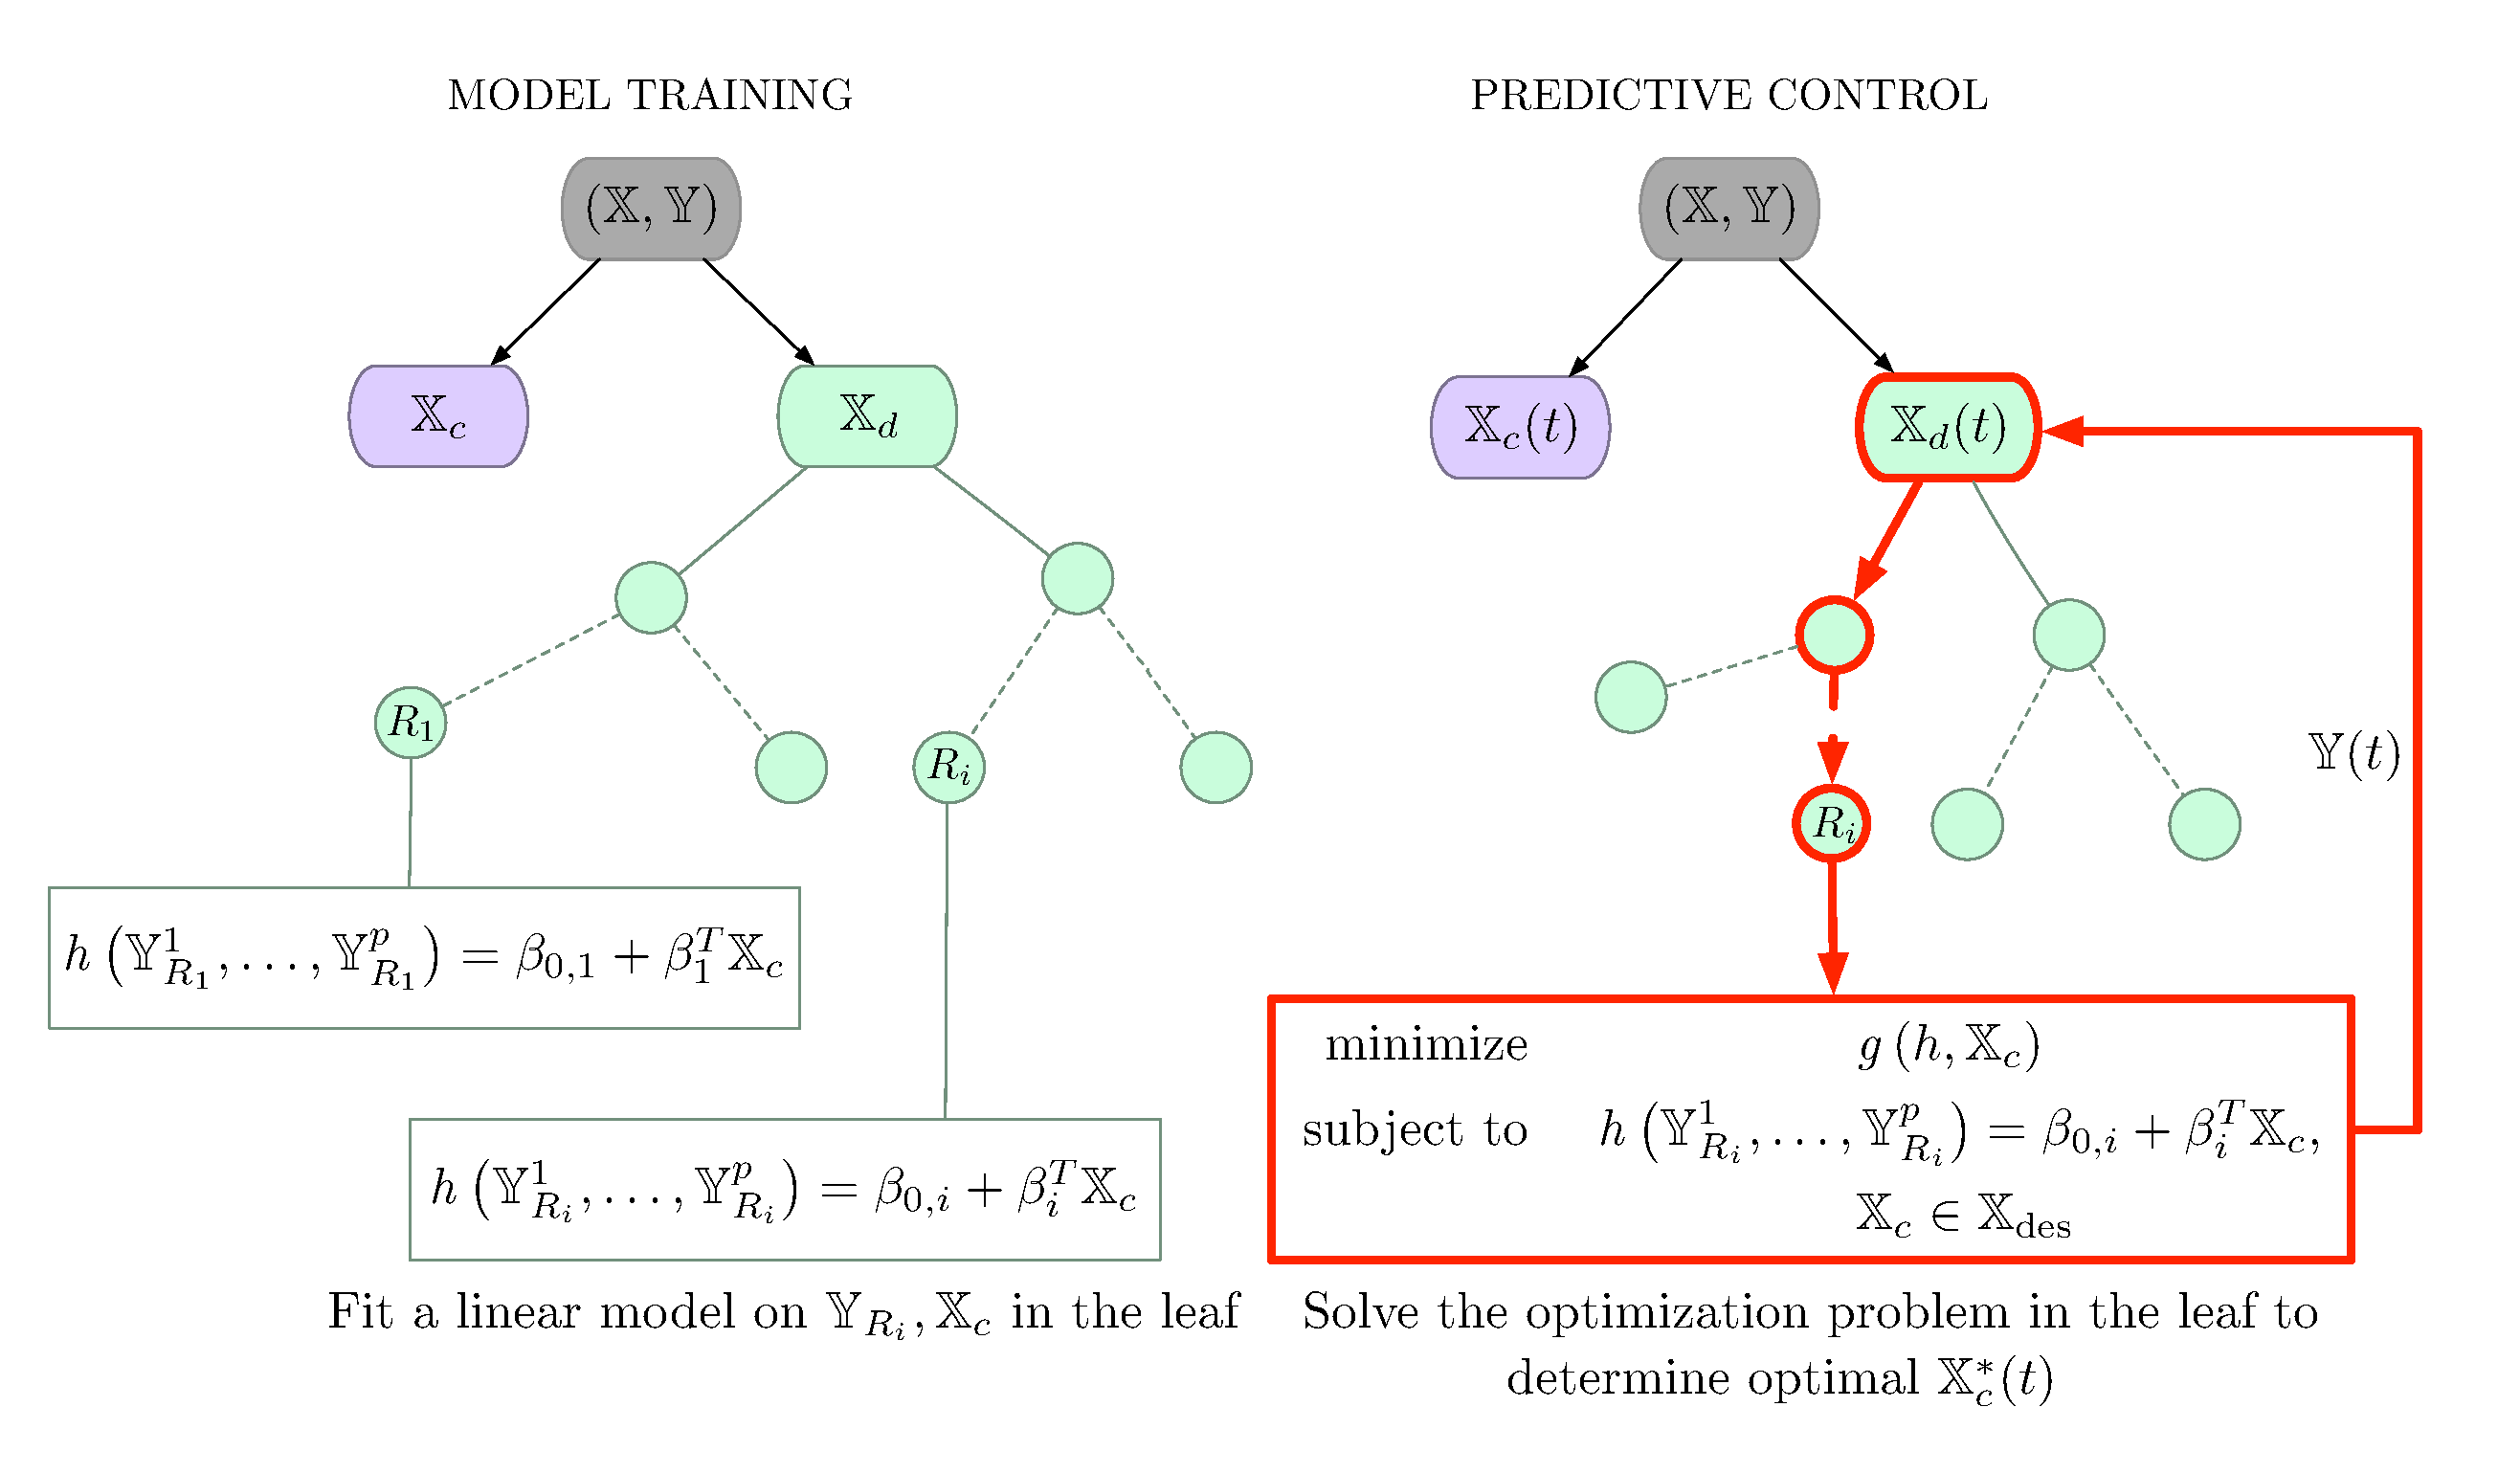
\includegraphics[width=0.9\linewidth]{Figures/DPC_tree2.eps}
	\caption{Data Predictive Control with Regression Trees with Model Training Process (left) and Receding Horizon Control (right). During the control step, the optimal control sequence $\left[u^*_t,\dots,u^*_{t+N}\right]^\top $ is determined. The first input $u(t)=u^*_t$ is applied to the system. The resulting output $\y_t$ which is a feature for the next time step is fed back to determine to determine $R_{i}$ at $t+1$.}
	\captionsetup{justification=centering}
	\label{F:DPC_schematic}
\end{figure*}
